
% 
% Annual Cognitive Science Conference
% Sample LaTeX Paper -- Proceedings Format
% 

% Original : Ashwin Ram (ashwin@cc.gatech.edu)       04/01/1994
% Modified : Johanna Moore (jmoore@cs.pitt.edu)      03/17/1995
% Modified : David Noelle (noelle@ucsd.edu)          03/15/1996
% Modified : Pat Langley (langley@cs.stanford.edu)   01/26/1997
% Latex2e corrections by Ramin Charles Nakisa        01/28/1997 
% Modified : Tina Eliassi-Rad (eliassi@cs.wisc.edu)  01/31/1998
% Modified : Trisha Yannuzzi (trisha@ircs.upenn.edu) 12/28/1999 (in process)
% Modified : Mary Ellen Foster (M.E.Foster@ed.ac.uk) 12/11/2000
% Modified : Ken Forbus                              01/23/2004
% Modified : Eli M. Silk (esilk@pitt.edu)            05/24/2005
% Modified : Niels Taatgen (taatgen@cmu.edu)         10/24/2006
% Modified : David Noelle (dnoelle@ucmerced.edu)     11/19/2014
% Modified : Elisa Kreiss (ekreiss@uos.de)    10/10/2016

%% Change ''letterpaper'' in the following line to ''a4paper'' if you must.

\documentclass[10pt,letterpaper]{article}

\usepackage{cogsci}
\usepackage{pslatex}
\usepackage{apacite}
\usepackage{amsmath,amssymb}
\usepackage{graphicx}
\usepackage{color}
\usepackage{url}
\usepackage{todonotes}
\usepackage{mathtools}
\usepackage{stmaryrd}
\usepackage{booktabs}
\usepackage{array}

\newcommand{\den}[2][]{
\(
\left\llbracket\;\text{#2}\;\right\rrbracket^{#1}
\)
}

%\newcommand{\url}[1]{$#1$}


\definecolor{Blue}{RGB}{0,0,255}
\definecolor{Green}{RGB}{10,200,100}
\definecolor{Red}{RGB}{255,0,0}
\newcommand{\jd}[1]{\textcolor{Blue}{[jd: #1]}}  
\newcommand{\rdh}[1]{\textcolor{Red}{[rdh: #1]}}  
\newcommand{\red}[1]{\textcolor{Red}{#1}}
\newcommand{\ndg}[1]{\textcolor{Green}{[ndg: #1]}}

 \newcommand{\denote}[1]{\mbox{ $[\![ #1 ]\!]$}}


\newcommand{\subsubsubsection}[1]{{\em #1}}
\newcommand{\eref}[1]{(\ref{#1})}
\newcommand{\tableref}[1]{Table \ref{#1}}
\newcommand{\figref}[1]{Fig.~\ref{#1}}
\newcommand{\appref}[1]{Appendix \ref{#1}}
\newcommand{\sectionref}[1]{Section \ref{#1}}

\title{Mentioning atypical properties of objects is communicatively efficient}

 
\author{{\large \bf Elisa Kreiss, Judith Degen, Robert X.D. Hawkins, Noah D.~Goodman} \\
  ekreiss@uos.de, \{jdegen,rxdh,ngoodman\}@stanford.edu\\
  Department of Psychology, 450 Serra Mall \\
  Stanford, CA 94305 USA}



\begin{document}

\maketitle


\begin{abstract}


\textbf{Keywords:} 
keywords
\end{abstract}

%\section{\bf Introduction}

Reference to objects is one of the most basic functions of language. How do speakers decide which of an object's properties to include in a referring expression? This problem of content selection (\jd{cite the dutch}) has plagued cognitive science for decades. For example, in Fig.~1c, the utterances `blue banana', `banana', `blue fruit', etc.~all uniquely establish reference to the same target: the blue banana. How do speakers decide between these? One factor that has been identified as affecting speakers' choice of referring expression is the expression's \emph{contextual informativeness}. Assuming that properties either do or do not apply to objects, `banana' would be the appropriate choice in Fig.~1c (where no other banana competes with the target banana), but `blue banana' when there is also a competing brown banana (as in Fig.~1b). However, previous research has established that this is not the case: speakers generally prefer to mention properties of objects to the extent that they are atypical, even when doing so is unnecessary for uniquely establishing reference \cite{sedivy2003a, Mitchell2013, westerbeek2015, rubiofernandez2016}. That is, speakers are more likely to redundantly call a blue banana `blue banana' but a yellow banana simply `banana'. Why is this so?

%The banana itself is a color-diagnostic object (Tanaka and Presnell, 1999), meaning different colors can have differently strong associations with, or be differently symptomatic of the object. A banana is normally associated with being yellow, a bit less with being brown, and not at all with being blue. When rating the association between the object and its color, we talk about \textit{typicality}. For a cup, all colors have approximately the same typicality, and it is therefore a non-color-diagnostic object.\\

%Various studies (Westerbeek, Mitchell, …) have shown that the color of a color-diagnostic object governs the chosen referring expression significantly. Westerbeek (cite) looked at contexts in which the referred-to object can unambiguously be distinguished from the other objects by only mentioning the type. Additionally, there has always been one object present that had the same color as the target (similar to Fig.~1d). Therefore, only considering unambiguous reference expressions, the use of color terms in any way would be “overinformative”, i.e., a true but unnecessarily added information. Westerbeek (cite) found that the lower the typicality for a color given the referred-to object is, the more likely one is to mention the color overinformatively.\\

%Looking at the example from the beginning again, Westerbeek's result would suggest that people would also tend to say 'blue banana'  in Fig.~1c to refer to the target object even if 'banana' would already be a sufficient way to do so.\\

An account of why more typical properties are less likely to be mentioned is still lacking. Some (\jd{cite}) have proposed that it is due to a speaker-internal pressure to mention salient properties; others (\jd{cite}) have proposed that speakers mention properties to facilitate the listener'��s visual search. Here, we ask the computational-level question: when should a rational speaker with the goal of correctly communicating the intended referent be expected to mention an object's color?

Following the bulk of the previous literature, we assume that a speaker's choice of referring expression is governed by multiple factors, including the expression's contextual informativeness and its cost. Following  \citeA{GrafEtAl2016,DegenEtAl-inprep} \jd{who else?}, we model speaker behavior formally within the Rational Speech Act (RSA) framework \cite{frank2012, GoodmanFrank2016}. However, we show that with a deterministic semantics for nouns and color adjectives, RSA cannot capture typicality effects in language. Therefore, also following \citeA{GrafEtAl2016,DegenEtAl-inprep}, we allow the semantics of expressions to assume a continuous value. That is, we allow `banana'-hood or `blue'-ness to apply to a given object to some degree rather than deterministically. This change directly affects expressions' contextual informativeness, resulting in precisely the expected typicality effects, as we demonstrate below.

In order to quantitatively evaluate the model, we collected freely produced referring expressions to objects in a web-based two-player reference game experiment (see \figref{fig:mturk}). We presented participants with color-diagnostic objects that varied in how typical their colors were. Objects were presented in different contexts to vary the contextual informativeness of mentioning color (see \figref{fig:contexts}). \jd{continue here} 

%One of the two players was given the role of the listener, the other one the role of the speaker. They could communicate freely with each other through a chat box which ensured natural language data. In each context, both saw the same objects but only the speaker had the special marking of the referent which he had to communicate to the listener. The listener then had to deduce the correct target from the speaker’s utterance and mark it by clicking on the object. 
%The context were manipulated by a differing typicality for the target object, and by distractor variation (either sharing the target's type, color or none of those). This way we could evaluate the effect of typicality and different kinds of contexts on referring expressions.

We expected to replicate color typicality effects on referring expressions in at least those contexts where color use would be `overinformative' (Fig.~1c) and 1d)), i.e., not strictly necessary for uniquely establishing reference. We included contexts in which mentioning color was informative (Fig.~1a) and 1b)) as a control condition as well as to test (to our knowledge, for the first time) whether typicality effects are observed even in situations where mentioning color is seemingly necessary for uniquely establishing reference.

\begin{figure}
	\centering
	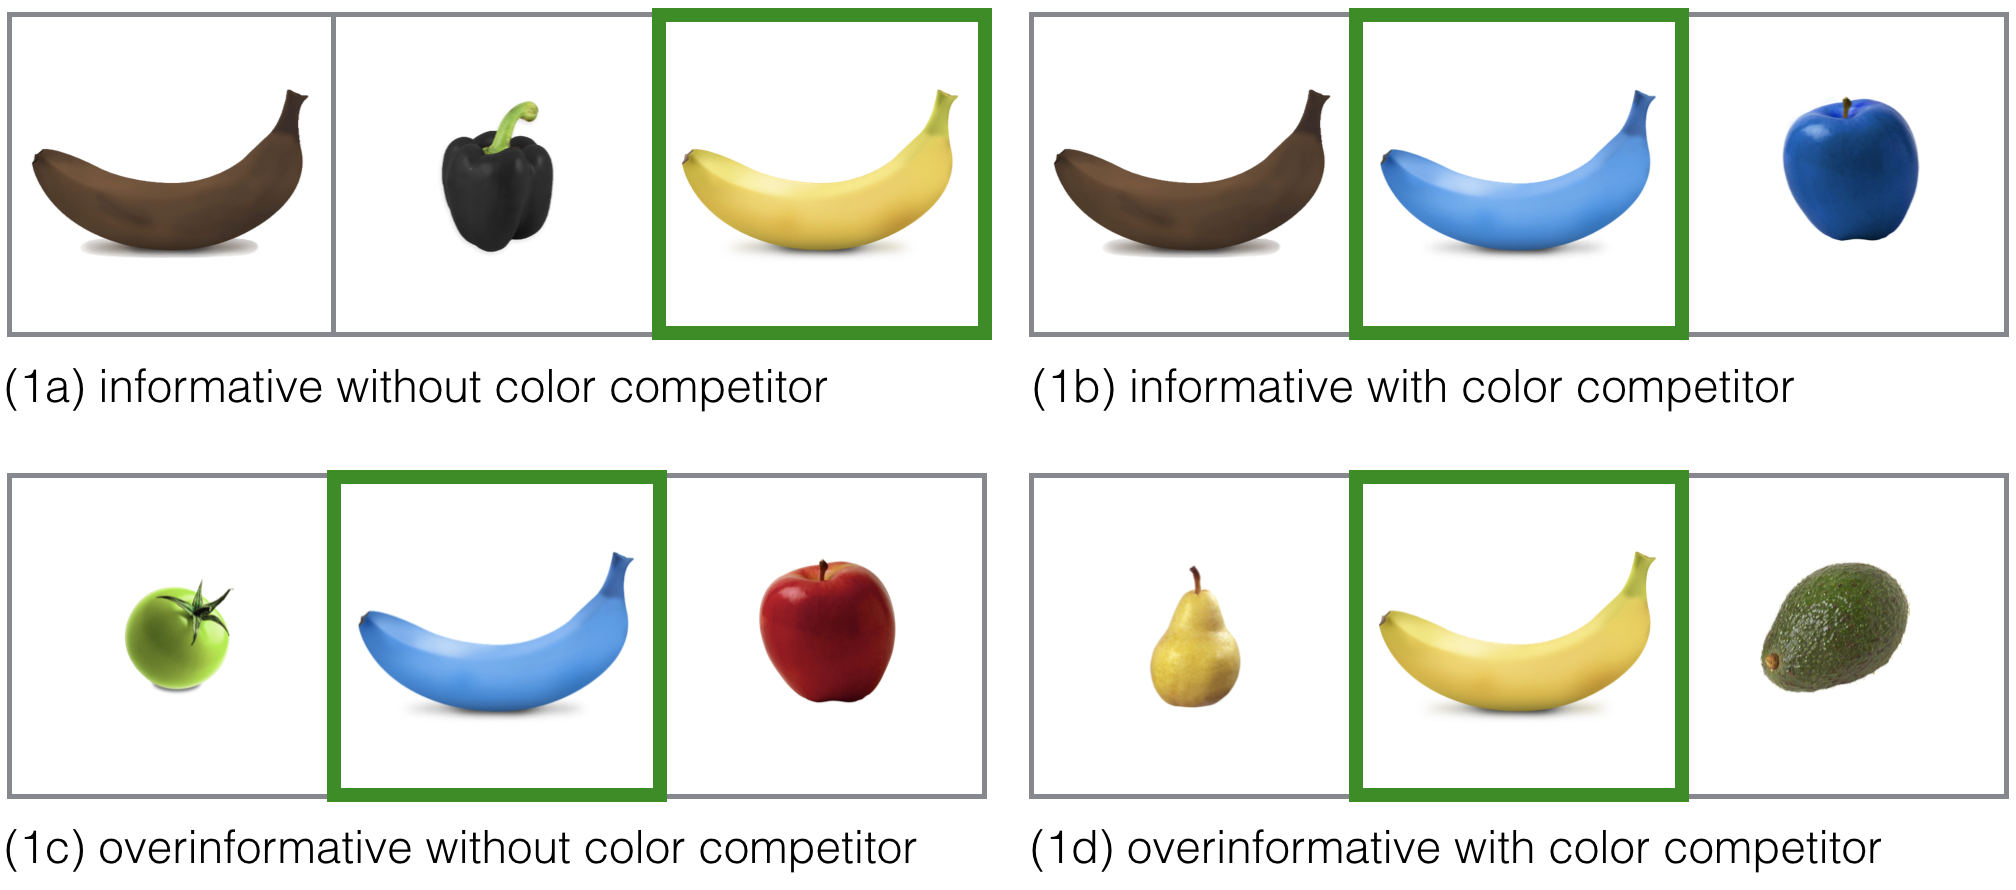
\includegraphics[width=.5\textwidth]{graphs/context_overview}
	\caption{The four context conditions, exemplified by the \textit{banana} domain. The target is outlined in green; the color and type of the distractors differ with each condition (see text).
	}
	\label{fig:contexts}
\end{figure}

We first report the production experiment. We then report norming studies we conducted to empirically elicit typicality values for all utterance-object pairs. We then report a comparison of different RSA models with graded semantics against a deterministic semantics baseline. Model comparison makes use of the empirically elicited typicality values to derive behavioral predictions, which we compare against the data obtained in the reported production experiment.

%In this paper, we also describe how this effect can be modeled by using the Rational-Speech-Acts (RSA) framework (Frank \& Goodman, 2012; Goodman \& Stuhlmüller, 2013). This model already showed good performance in various language interpretation tasks (e.g. Goodman \& Stuhlmüller, 2013; Kao, Wu, Bergen, \& Goodman, 2014), but has only recently been applied to production data(, also with promising results???) (but see Franke, 2014; Orita, Vornov, Feldman, \& Daume ́ III, 2015, Graf, 2016). 
%A speaker in RSA is treated as an approximately optimal decision maker who chooses which utterance to use to communicate to a listener. The speaker has a utility which includes terms for the cost of producing an utterance (in terms of length or frequency) and the informativeness of the utterance for a listener. The listener is treated as a literal Bayesian interpreter who updates her beliefs given the truth of the utterance. These truth values are usually treated as deterministic (an object either is a “dog” or it is not); here we relax this formulation in order to incorporate typicality effects. That is, we elicit typicality ratings in a separate experiment, and model the listener as updating her beliefs by weighting the possible referents according to how typical each is for the description used. We evaluate the quantitative model predictions against our production data. The model also allows us to evaluate the need for each extra component—typicality, length, frequency—and determine whether the empirical bias toward reference at the basic level (Rosch et al., 1976) can be accounted for without build- ing it in as a separate factor.  (from Caroline)\\
%In this particular case, the RSA model can capture the effects of the context on the reference production, and the typicality effect.

\section{Experiment: color reference game}

\begin{figure}[bt!]
	\centering
	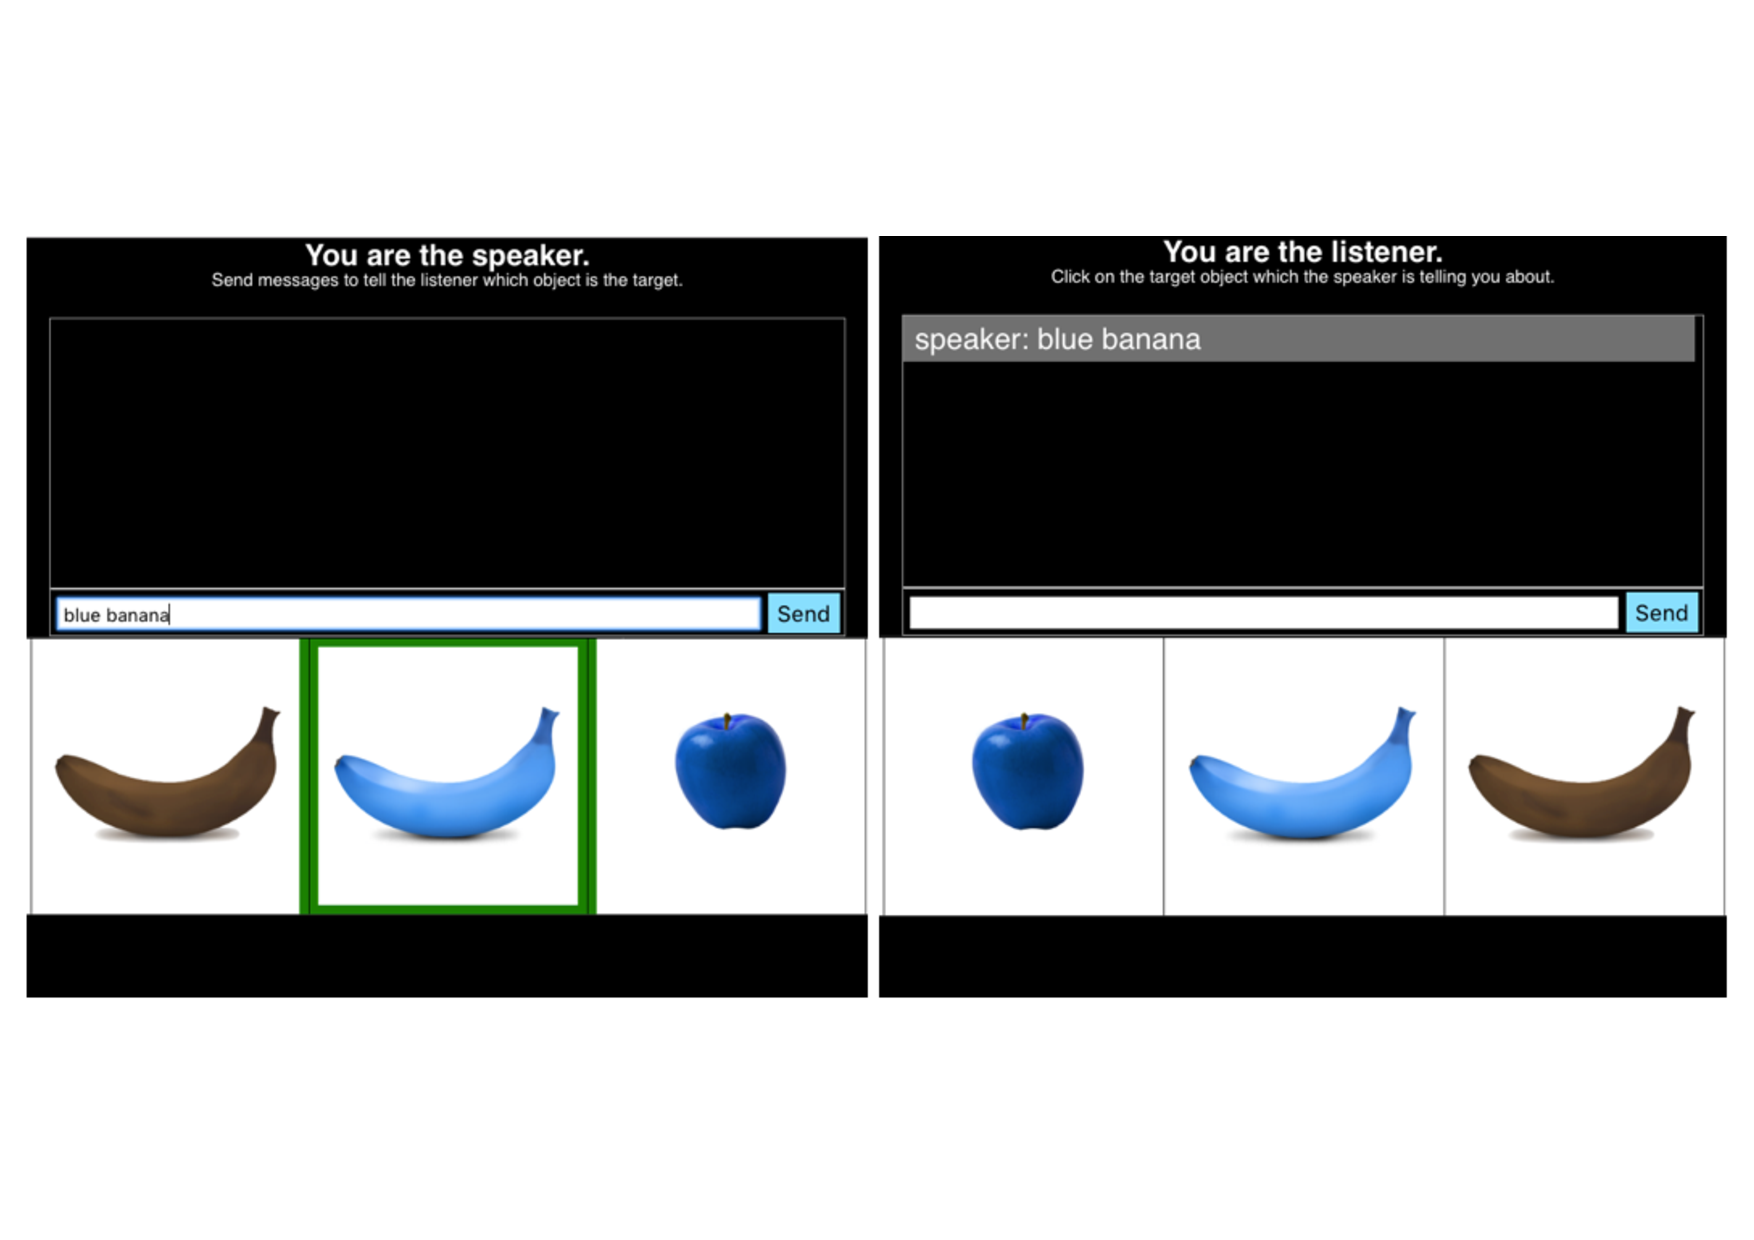
\includegraphics[width=.5\textwidth]{graphs/design_0}
	\caption{Experimental setup.
	}
	\label{fig:mturk}
\end{figure}

\subsection{Methods}

\paragraph{Participants and materials}
We recruited 120 self-reported native speakers of English over Mechanical Turk. The experiment was a multi-player reference game in which one participant was randomly assigned to the role of the speaker, and the other one to the role of the listener. The speaker's task was to communicate a target object out of three-object contexts to the listener. The target was always marked with a green border (see \figref{fig:mturk}). The listener clicked on the object they thought was the target. The speaker and the listener could communicate freely through a chat box.

%\paragraph{\bf Materials}
The stimuli were selected from seven food items which each occurred in three different colors, e.g., one of the seven food items was the banana that occurred in the colors yellow, brown, and blue. All of those stimuli occurred as targets and distractors. A pepper additionally occurred in a fourth color which only functioned as a distractor due to the need for an adequate green color competitor.

%\paragraph{\bf Design}
Each presented context consisted of three objects, one target and two distractors. The contexts always corresponded to one out of four possible conditions. The different context conditions are referred to as ``informative without a color competitor" (Fig.~1a), ``informative with a color competitor" (Fig.~1b), ``overinformative without a color competitor" (Fig.~1c), and ``overinformative with a color competitor" (Fig.~1d). A context is referred to as overinformative when mentioning the type of the item, e.g., banana, would be sufficient for an unambiguous identification of the target. An additional mention of color would mean that the speaker uses the color adjective overinformatively, i.e., they are adding ``unnecessary" information. However, in this condition the target never has a color competitor, i.e., if the target is brown, there is no distractor of the same color in the context. This means that an only-color utterance would lead to an unambiguous identification, too. This is not possible in the overinformative condition with a color competitor (Fig.~1d). In the informative conditions, the speaker needed to mention the color in addition to the type to provide an unambiguous utterance. Again, one context type did (Fig.~1a) and one did not include a color competitor among its distractors (Fig.~1b).

The item selection was randomized but conditioned on the corresponding context condition, i.e., the items had to fulfill the properties dictated by the condition. In the end, each participant saw 42 different contexts. All of the differently colored items were the target exactly twice but the context in which they occurred was drawn randomly from the four possible conditions mentioned above. All in all, there were 84 different configurations, i.e., seven target food items, each of them in three colors, where each could occur in four contexts. Trial order was randomized.


\paragraph{Procedure}

Participants were randomly paired up and each was randomly assigned either to the role of  speaker or listener. They communicated through a real-time multi-player interface as described in \citeA{hawkins2015}. The virtual environment of the experiment can be seen in \figref{fig:mturk}. The speaker and the listener saw the same set of objects but in a randomized order to avoid trivial position-based references such as ``the left one". After the listener clicked on the presumed target, both speaker and listener received feedback about whether the right object had been selected.


\paragraph{Annotation}
After collecting the data, the different utterances were labeled as belonging to one of the following categories: type-only ("banana"), color-and-type ("yellow banana"),  color-only ("yellow"), category-only ("fruit"), color-and-category ("yellow fruit"), description ("has green stem"), color-modifier ("funky carrot"), and negation ("yellow but not banana"). Before sorting, two participants had to be excluded because they did not finish the experiment, and therefore could not be paid. Furthermore, trials in which the speaker did not produce any utterances, and trials in which the listener could not identify the target correctly were excluded, too. The remaining utterances (94\% of the original set) were cleaned manually for misspellings and abbreviations, e.g., ``banan" for banana. Afterwards, the speakers that continuously refused to name objects but used unnatural descriptions instead (e.g., "monkeys love..." for banana) were excluded, too, as they misunderstood the task and the resulting expressions were therefore not relevant for the study.

The resulting utterances were then categorized according to the categories laid out above. Only five utterances (0.003\%) were assigned to the category "other".

\begin{figure}[bt!]
	\centering
	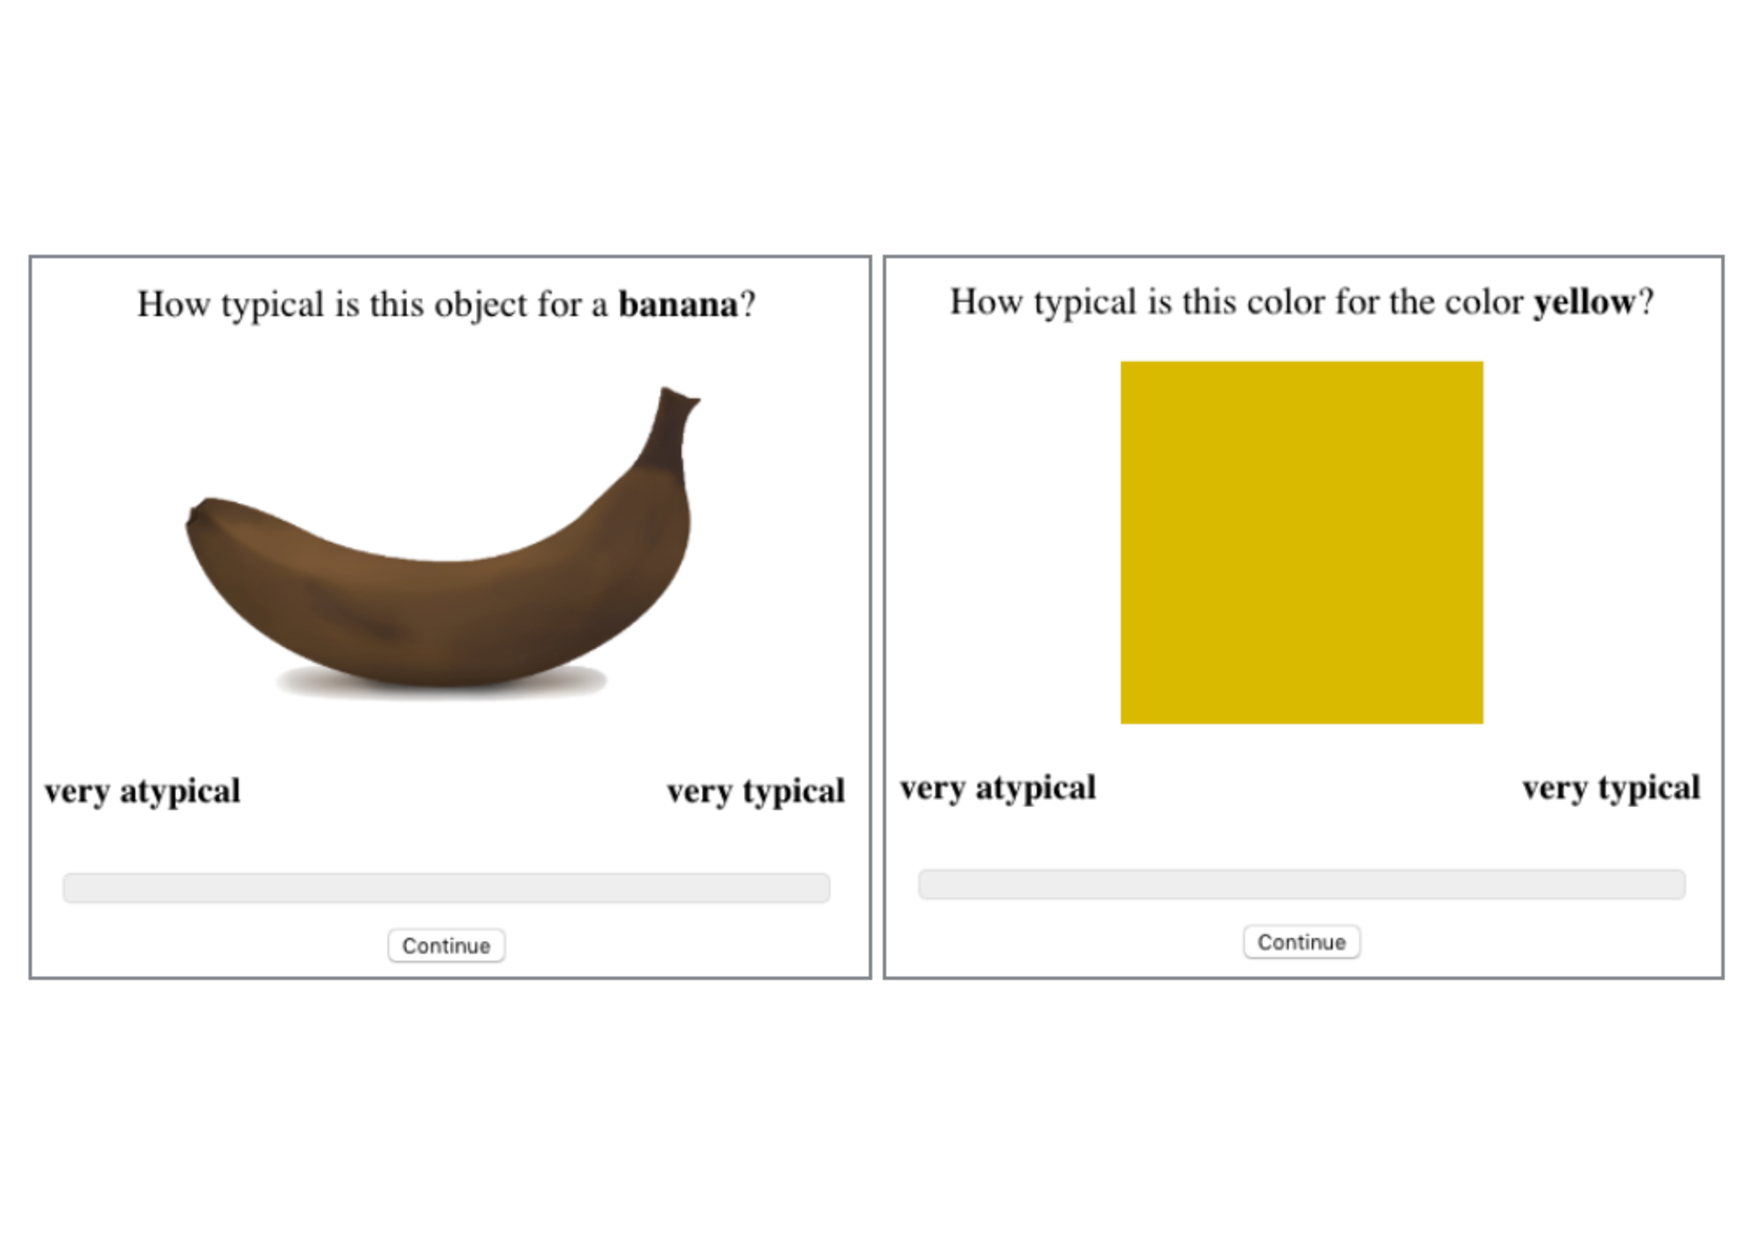
\includegraphics[width=.5\textwidth]{graphs/design_2}
	\caption{Typicality norming studies for object and color patch norming.
	}
	\label{fig:design_2}
\end{figure}

\begin{figure}[bt!]
	\centering
	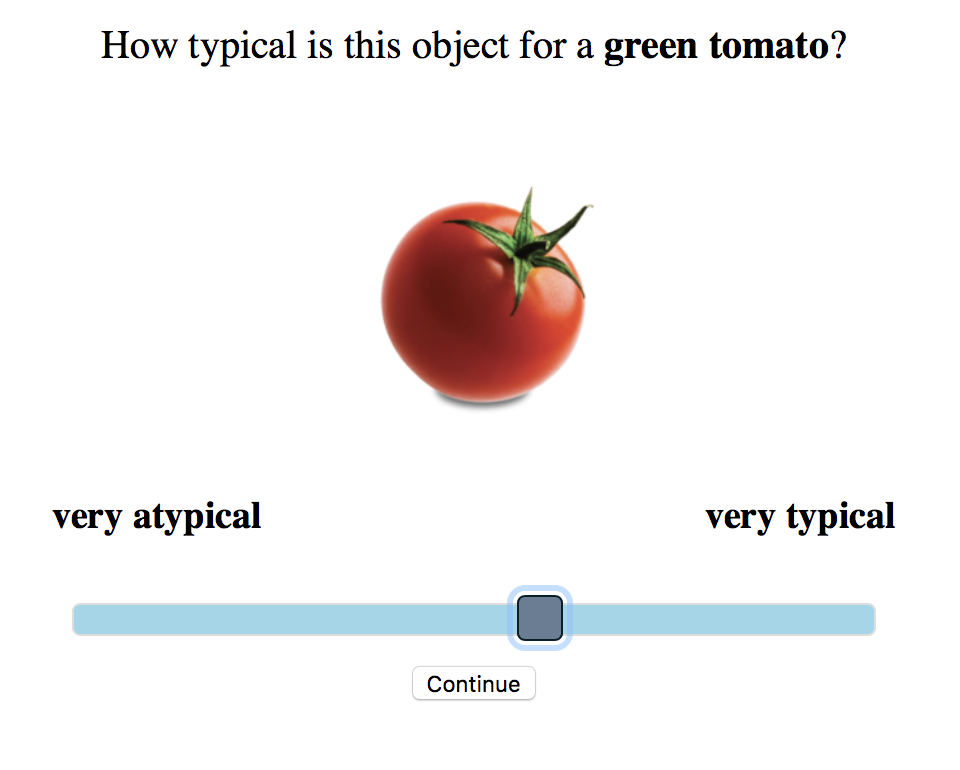
\includegraphics[width=.5\textwidth]{graphs/typ_norm_full_2}
	\caption{Typicality norming study.
	}
	\label{fig:typ_norm_full_2}
\end{figure}

\paragraph{Typicality norming}
For further analysis of the objects, we conducted two norming studies - an object and a color norming study. Both had 75 participants that were recruited over Mechanical Turk.

In the object norming study, the participants were shown a colored food item, e.g., a blue banana, and asked "How typical is this object for an X?" (X being a type, e.g., banana, or a category, e.g., fruit). The participants could rate the fitness on a continuous draggable scale from "very atypical" to "very typical". Every object in the set was paired with every type and category expression from the set, resulting in 189 different trials.

The aim of the color norming study was to identify how typical a certain object's color is for different color terms, i.e., how blue is the given color. The color patches were constructed by determining the average color of the object, stems and leaves excluded. The participants were presented with this color patch, and had to rate its typicality given a certain color term. Again, they had a continuous draggable scale with the end marks "very atypical" and "very typical". Eight color terms were paired with 21 color patches and which resulted in 168 trials.

Due to the amount of trials, each participant only saw a subset of 90. The decision on which trials were shown was random with a slight preference on fitting combinations, e.g., seeing a blue banana and asking for "banana", in contrast to seeing a blue carrot and asking for "apple". The amount of data per combination ranged from 13 to 60. The assumed typicality values are the averaged slider values for each combination ranging from 0.004 (very atypical) to 0.989 (very typical). 

To get empirical typicality values of the objects, we conducted a norming study. 64 participants (2 excluded because of random clicking, 2 excluded because of non-English speakers) have been recruited via Mechanical turk. 
They were shown a colored food item, e.g., a blue banana, and asked "How typical is this object for an X?" (X being a color-type combination, e.g., blue banana, or red apple). The participants could rate the fitness on a continuous draggable scale from "very atypical" to "very typical". Every object in the set was paired with every color-type combination from the set, resulting in 484 different trials. Each participant answered 110 trials in which type consistent trials (showing all kinds of bananas when utterance contains banana) were always present, and non-fitting trials which were selected randomly. The amount of data per combination ranged from ... to ... . The assumed typicality values are the averaged slider values for each combination ranging from 0 (very atypical) to 0.968 (very typical). 

\subsection{\bf Results}

\jd{judith needs to fill this in}

%Proportions of sub, basic, and super level utterance choices in the different context conditions are shown in the top row of \figref{fig:qualitativemodel}. The sub level term was preferred where it was necessary for unambiguous referent identification, i.e., when a distractor of the same basic level category as the target was present in the scene (item12, e.g. target: dalmatian, distractor: greyhound). Where it was not necessary (i.e., when there was no other object of the same basic level category present, as in conditions item22, item23 and item33), there was a clear preference for the basic level term. The super level term was strongly dispreferred overall, though it was used on some trials, especially where informativeness constraints on utterance choice were weakest (item33). 
%To test for the independent effects of informativeness, length, frequency, and typicality on sub-level mention, we conducted a mixed effects logistic regression. Frequency was coded as the difference between the sub and the basic level's log frequency, as extracted from the Google Books Ngram English corpus ranging from 1960 to 2008. Length was coded as the ratio of the sub to the basic level's length.\footnote{We used the mean empirical lengths in characters of the utterances participants produced. For example, the minivan, when referred to at the subcategory level, was sometimes called ``minivan'' and sometimes ``van'' leading to a mean empirical length of 5.64. This is the value that was used, rather than 7, the length of ``minivan''.} That is, a higher frequency difference indicates a \emph{lower} cost for the sub level term compared to the basic level, while a higher length ratio reflects a \emph{higher} cost for the sub level term compared to the basic level.\footnote{We replicate the well-documented negative correlation between length and log frequency ($r = -.53$ in our dataset).} Typicality was coded as the ratio of the target's sub to basic level label typicality. That is, the higher the ratio, the more typical the object was for the sub level label compared to the basic level.
%For instance, the panda was relatively atypical for its basic level ``bear'' (mean rating 0.75) compared to the sub level term ``panda bear'' (mean rating 0.98), which resulted in a relatively \emph{high} typicality ratio.

\begin{figure}[bt]
\centering
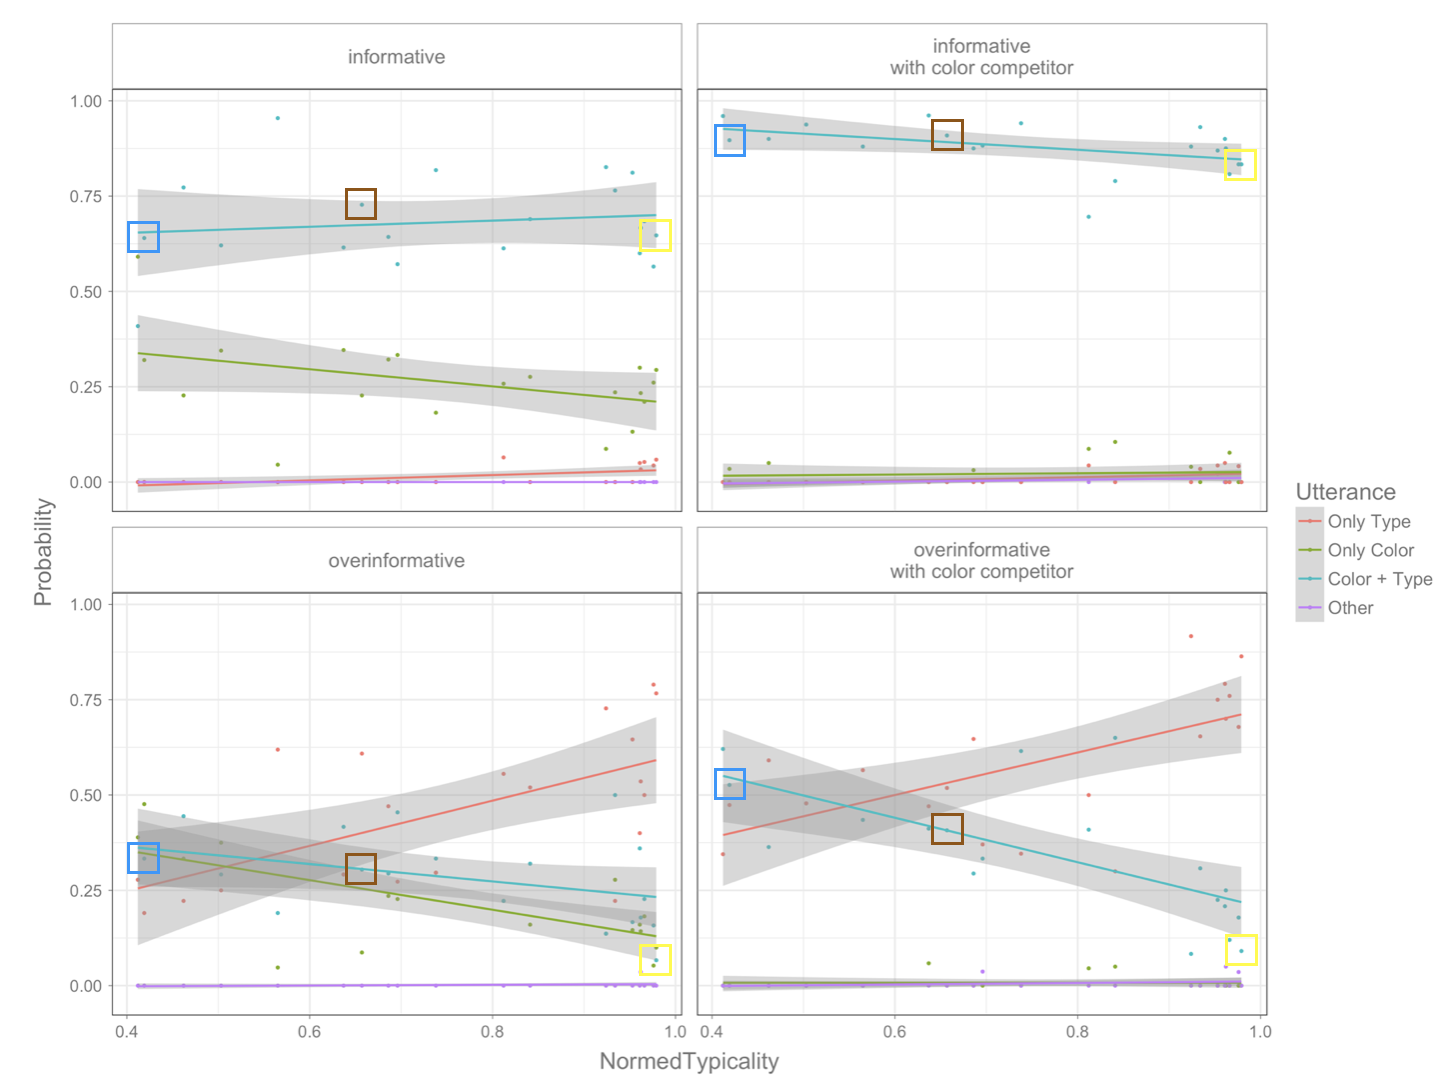
\includegraphics[width=.5\textwidth]{graphs/cuny_graph}
\caption{Proportion of Color ("blue"), Type ("banana"), and ColorAndType ("blue banana") utterances as a function of mean object typicality ???for the Type utterance???, across conditions. "COLOR banana" cases are circled in their respective color.}
\label{fig:qualitativemodel}
\end{figure}

%Condition was coded as a three-level factor: \emph{sub necessary}, \emph{basic sufficient}, and \emph{super sufficient}, where item22 and item23 were collapsed into \emph{basic sufficient}. Condition was Helmert-coded: two contrasts over the three condition levels were included in the model, comparing each level against the mean of the remaining levels (in order: \emph{sub necessary}, \emph{basic sufficient}, \emph{super sufficient}). This allowed us to determine whether the probability of type mention  for neighboring conditions were significantly different from each other, as suggested by \figref{fig:qualitativemodel}.\footnote{Adding terms that code the ratio of the sub vs super level frequency and length did not lead to an improvement of model fit.} The model included random by-speaker and by-domain intercepts. 
%
%A summary of results is shown in \tableref{tab:modelresults}. The log odds of mentioning the sub level term was greater in the \emph{sub necessary} condition than in either of the other two conditions, and greater in the \emph{basic sufficient} condition than in the \emph{super sufficient} condition, suggesting that the contextual informativeness of the sub level mention has a gradient effect on utterance choice.\footnote{Importantly, model comparison between the reported model and one that subsumes basic and super under the same factor level revealed that the three-level condition variable is justified ($\chi ^2 (1) = 5.7$, $p < .05$), suggesting that participants don't simply revert to the basic level unless contextually forced not to.} There was also a main effect of typicality, such that the sub level term was preferred for objects that were more typical for the sub level compared to the basic level  description (\figref{fig:lengthtypicality}). In addition, there was a main effect of length, such that as the length of the sub level term increased compared to the basic level term (``chihuahua''/``dog'' vs.~``pug''/``dog''), the sub level term was dispreferred (``chihuahua'' is dispreferred compared to ``pug'', \figref{fig:lengthtypicality}). Finally, while there was no main effect of frequency, we observed a significant length by frequency interaction, such that there was a frequency effect for the relatively shorter but not the relatively longer sub level cases: for shorter sub level terms, relatively high-frequency sub level terms were more likely to be used than relatively low-frequency sub level terms. 

%\begin{table}[tbp]
%\caption{Mixed effects model summary.}
%\begin{center}
%\begin{tabular}{lrrl}
%\toprule
%\multicolumn{1}{l}{}&\multicolumn{1}{c}{Coef $\beta$}&\multicolumn{1}{c}{SE($\beta$)}&\multicolumn{1}{c}{$p$}\tabularnewline
%\midrule
%Intercept&$-0.30$&$0.35$&\textgreater0.4\tabularnewline
%Condition sub.vs.rest&$ 2.46$&$0.24$&\textbf{\textless.0001}\tabularnewline
%Condition basic.vs.super&$ 0.52$&$0.23$&\textbf{\textless.05}\tabularnewline
%Length&$-0.52$&$0.14$&\textbf{\textless.001}\tabularnewline
%Frequency&$-0.02$&$0.08$&\textgreater0.78\tabularnewline
%Typicality&$ 4.17$&$0.84$&\textbf{\textless.0001}\tabularnewline
%Length:Frequency&$-0.30$&$0.11$&\textbf{\textless.01}\tabularnewline
%\bottomrule
%\end{tabular}\end{center}
%\label{tab:modelresults}
%\end{table}

%Unsurprisingly, there was also significant by-participant and by-domain variation in the log odds of sub level term mention. %\figref{fig:bigscatterplot} shows the by-domain variation in utterance choice. 
%For instance, mentioning the subclass over the basic level term was preferred more in some domains (e.g. in the ``candy'' domain) than in others. Likewise, some domains had a greater preference for basic level terms (e.g. the ``shirt'' domain). Using the superclass term also ranged from hardly being observable (e.g. the ``flower'' domain) to being used more frequently (e.g. in the ``bird'' domain). Nevertheless, mentioning the sub level term was always the most frequent choice where a distractor of the same basic level was displayed. Furthermore, it was the case in all domains that the sub level term was mentioned most frequently and the basic level least frequently in just this condition, compared to the other three conditions.
%

%\begin{figure}[bt]
%\centering
%%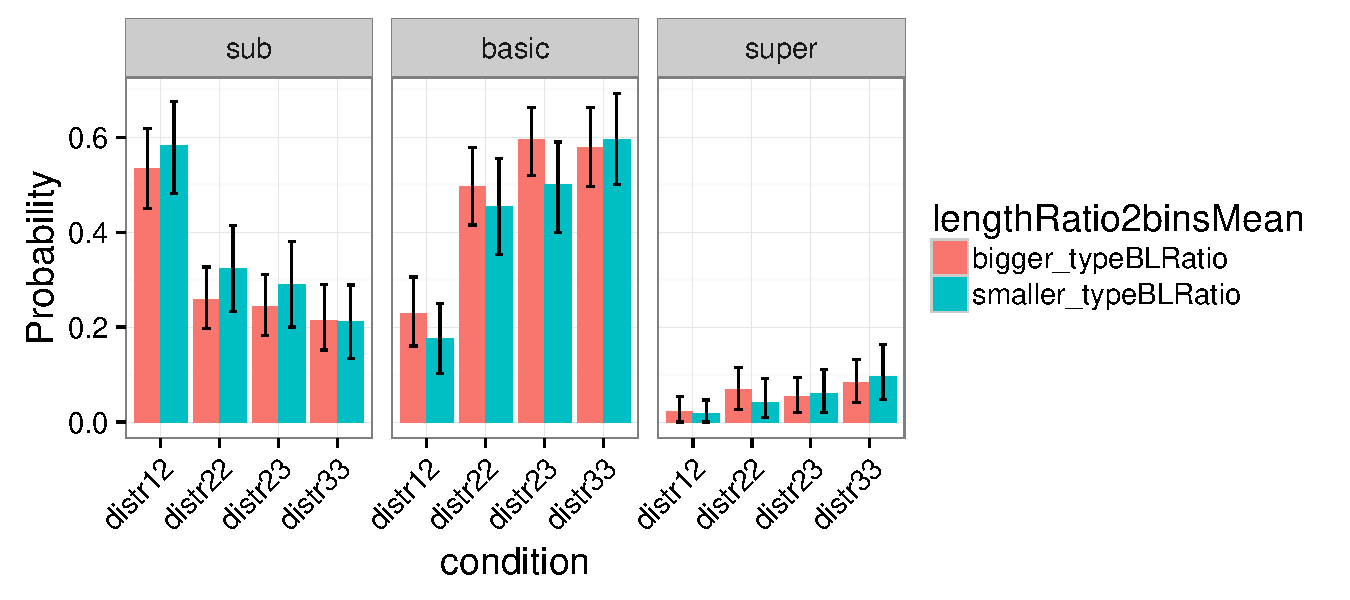
\includegraphics[width=.5\textwidth]{graphs/lengthRatio}
%%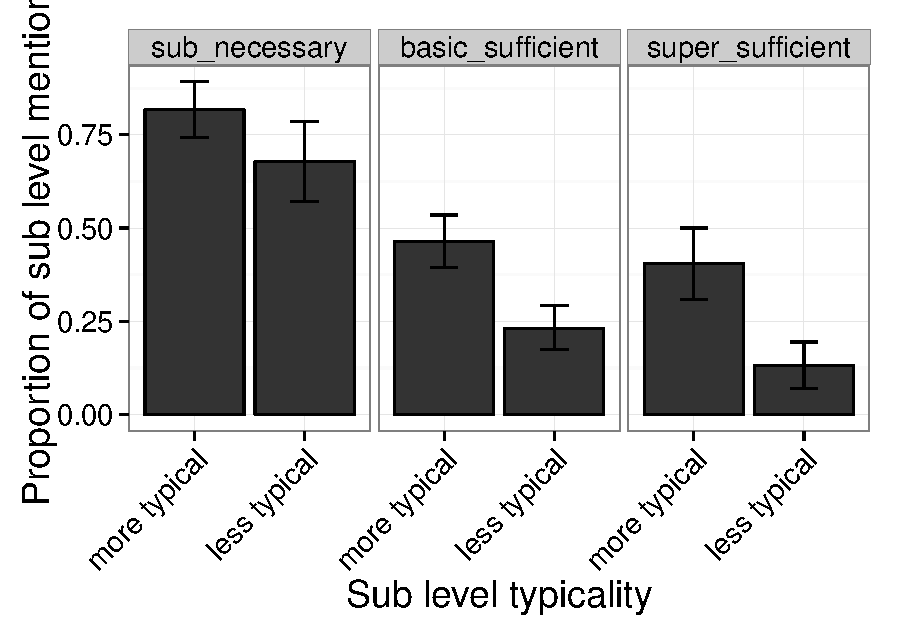
\includegraphics[width=.5\textwidth]{graphs/typicality-effect}
%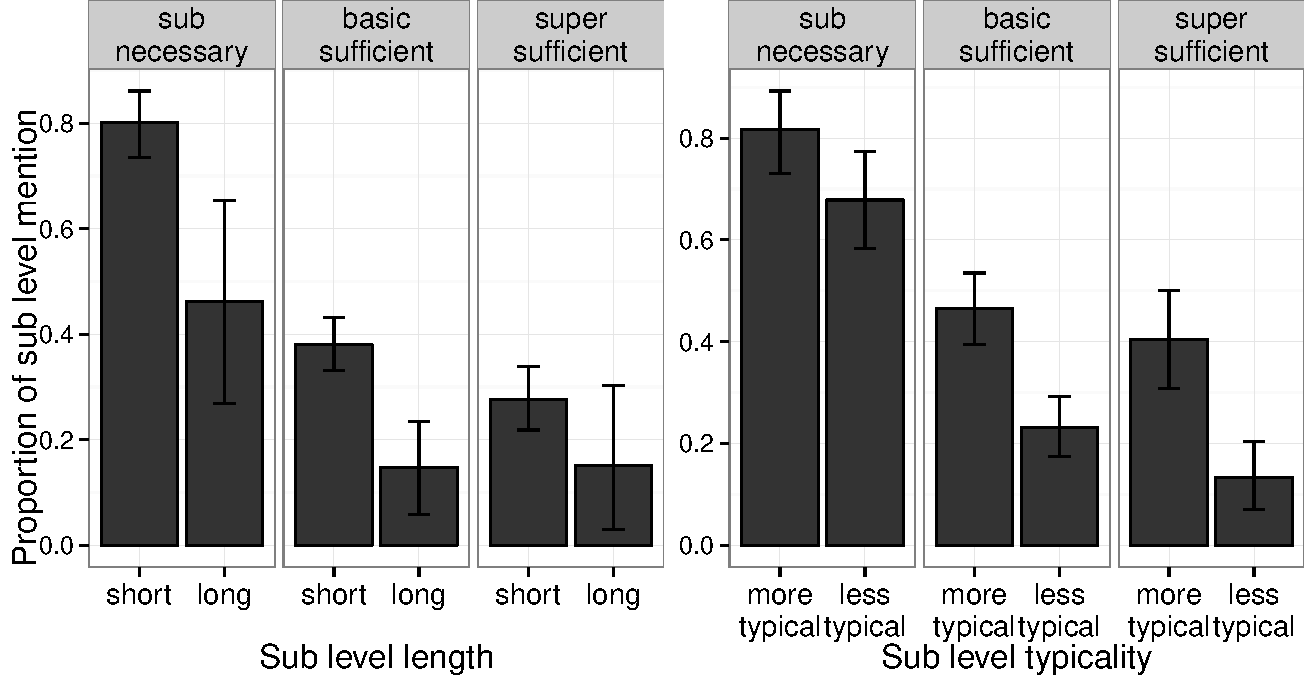
\includegraphics[width=.5\textwidth]{graphs/length-typicality}
%\caption{Probability of using sub, basic and super level terms. Left: when the sub  length is relatively short (.67,2] or long [2,4.67) compared to the basic level term length. Right: when the target object was relatively more [1.06,1.91) or less (.88,1.06] typical for the sub compared to the basic level term.}
% \label{fig:lengthtypicality}
%\end{figure}


\section{\bf Modeling referential expressions}

Next, we consider a family of computational models characterizing the communicative challenge a speaker agent faces in the reference game scenarios above. These models are all situated within the broader Rational Speech Act (RSA) framework, which has successfully explained a range of sophisticated language phenomena through a recursive process of social reasoning between speaker and listener agents \cite{frank2012, goodmanstuhlmueller2013, GoodmanFrank2016}. More formally, we define a \emph{literal listener} $L_0$ that selects between contextual referents $c \in \mathcal{C}$ proportionally to the meanings given by a lexicon $\mathcal{L}$:

$$L_0(c | u, \mathcal{C}) \propto \mathcal{L}(u, c) P(c)$$

We then introduce a pragmatic speaker $S_1$, which selects an utterance $u \in \mathcal{U}$ to communicate an intended referent $c_i$ by trading off \emph{informativity} with cost:
%%%
$$S_1(u | c_i) \propto \exp\left( \alpha\log(L_0(c_i | u, \mathcal{C})) - \textrm{cost}(u) \right)$$
%%%
where cost is usually defined as a function of an utterance's length or corpus frequency and $\alpha$ is a parameter controlling the speaker's ``optimality'': as $\alpha\rightarrow \infty$, they will choose utterances that maximize informativity. We explore several variations of this model in our model comparison, first considering different formulations of the lexicon $\mathcal{L}$ and then  several novel ways of enriching the speaker to marginalize over possible \emph{noise} in the listener's perception of the context:

\begin{description}

\item[Baseline:] The simplest version of the lexicon $\mathcal{L}$ uses truth-conditional meanings, such that a given utterance is either true or false of a given referent: $\mathcal{L}(u,c) = \delta_{u(c)}$. This is the traditional formulation in formal semantics, and the one most frequently used in previous RSA models. 

\item[Typicality:] Next, we consider the elaborated model in \citeA{GrafEtAl2016}, which focused on nominal reference contexts where a speaker must choose between different taxonomic levels of reference (e.g. `dalmatian,' `dog,' or `animal'). The primary innovation introduced by \citeA{GrafEtAl2016} was a shift to a graded, real-valued meaning function based on the \emph{typicality} of the referent relative to the utterance category: $\mathcal{L}(u,c) = \textrm{typicality(u, c)}$. This gives rise to phenomena where, for example, a speaker is more likely to use an overinformative utterance for a particularly atypical category member when a more typical referent is in context because they reason that $L_0$ would interpret the simpler utterance to mean the more typical referent. 

\item[Uniform Perceptual Noise:] We propose that perceptual noise is another critical factor in explaining the overproduction of redundant modifiers. In this variation of the model, the speaker supposes that with some noise parameter $p_{noise}$, the listener might have misperceived one or more of the objects in context, thus leading to a corrupted context $\mathcal{C}'$:
$$S_{noisy}(u|c_i) \propto \exp\left( \alpha\log\left(\sum_{\mathcal{C'}} P(\mathcal{C}')L_0(c_i | u, \mathcal{C}')\right) - \textrm{cost}(u)\right)$$
In the simplest version of this noisy-context model, the prior over possible misperceptions $P(\mathcal{C}')$ is uniform, such that the true context has probability $P(\mathcal{C}) = p_{noise}$, and the rest of the probability mass is spread evenly across all possible replacements of one or more objects $c \in \mathcal{C}$. Intuitively, this has the effect of making the speaker more cautious about using less specific utterances: even if there is only one `banana' in context, the speaker reasons that the listener may misperceive one of the distractors as another banana with some small probability, hence it may be useful to include a color modifier just in case.

\item[Similarity-Based Perceptual Noise:] This model is equivalent to the Uniform Perceptual Noise except for the prior $P(\mathcal{C'})$ over possible corruptions. Rather than choosing uniform across possible corruptions, we define a similarity metric such that misperceptions closer in similarity space to the true context (e.g. sharing one or more complete objects, only differing in color, and so on) are proportionally more likely: $P(\mathcal{C'}) \propto \textrm{sim}(\mathcal{C}, \mathcal{C'})$.
\rdh{Need to explain this similarity metric more once we've settled on one}
\end{description}

%The ghost-context model is similar to the simple model, but adds uncertainty by taking the true context and creating possible variants from it in a random fashion. This contributes the possibility of a misperception. Possible contexts that are more similar to the true context appear with a higher probability than those with a lower one. Here, similarity is only calculated on basis of the whole object (color and type) being identical to its corresponding partner in the true context
%This model also has an extended version in which the similarity measure is more fine-grained, i.e., color is not a binary feature anymore (either true or false) but rather can be more or less similar to the color of the object in the true context.







%
%We formulated a probabilistic model of reference level selection that integrates contextual informativeness, utterance cost, and typicality.
%As in earlier Rational Speech-Acts (RSA) models \cite{frank2012, goodmanstuhlmueller2013}, the speaker seeks to be informative with respect to an internal model of a literal listener. This listener updates her beliefs to rule out possible worlds that are inconsistent with the meaning of the speaker's utterance. Rather than assuming that words have deterministic truth conditions, as has usually been done in the past, we account for typicality by allowing each label a graded meaning. For instance, the word ``dog'' describes a dalmatian better than a grizzly bear, but it also describes a grizzly bear better than a tennis ball.
%The speaker also seeks to be parsimonious: the speaker utility includes both informativeness and word cost; cost includes both length and frequency.
%
%Formally, we start by specifying a literal listener $L_0$ who hears a word $l$ at a particular level of reference  in the context of some set of objects $\mathcal{O}$ and forms a distribution over the referenced object, $o \in \mathcal{O}$ : 
%$$P_{L_0}(o | l) \propto \denote{l}(o).$$
%Here $\denote{l}(o)$ is the lexical meaning of the word $l$ when applied to object $o$. We take this to be a real number indicating the degree of acceptability of object $o$ for category $l$. 
%We relate this to our empirically elicited typicality norms via an exponential relationship: $\denote{l}(o)=\exp(\text{typicality}(o,l))$.\footnote{Cases where typicality was not elicited were assumed to have typicality $0$.}
%This relationship is motivated by considering the effect of a small difference in typicality on choice probability: in our elicitation experiment a small difference in rating should mean the same thing at the top and bottom of the scale (it is visually equivalent on the slider that participants used).
%In order for a small difference in typicality rating to have a constant effect on relative choice probability (which is a ratio), the relationship must be exponential. 
%Next, we specify a speaker $S_1$ who intends to refer to a particular object $o \in \mathcal{O}$ and chooses among possible nouns $l \in {\mathcal L}(o)$.
%We take ${\mathcal L}(o)$ to be the three labels for $o$ at sub, basic, and super level.
%The speaker chooses among these nouns in a way that is influenced by informativeness of the noun for the literal listener ($\ln P_{L_0}(o | l)$), the frequency ($\hat{c}_f$) and the length  ($\hat{c}_l$), each weighted by a free parameter:
%$$P_{S_1}(l | o) \propto \exp(\lambda \ln P_{L_0}(o | l) + \beta_f \hat{c}_f  + \beta_l \hat{c}_l)$$
%Length cost $\hat{c}_l$ was defined as the empirical mean number of characters used to refer at that level and frequency cost $\hat{c}_f$ was the log frequency in the Google Books corpus from 1960 to the present. 
%
%We performed Bayesian data analysis to generate model predictions, conditioning on the observed production data (coded into sub, basic, and super labels as described above) and integrating over the three free parameters.
%We assumed uniform priors for each parameter: $\lambda  \sim Unif(0,20)$, $\beta_f \sim Unif(0,5)$, $\beta_l \sim Unif(0,5)$.
%We implemented both the cognitive and data-analysis models in the probabilistic programming language WebPPL \cite{GoodmanStuhlmuller14_DIPPL}.
%Inference for the cognitive model was exact, while we used Markov Chain Monte Carlo (MCMC) to infer posteriors for the three free parameters.

%\begin{figure}[t!]
%\centering
%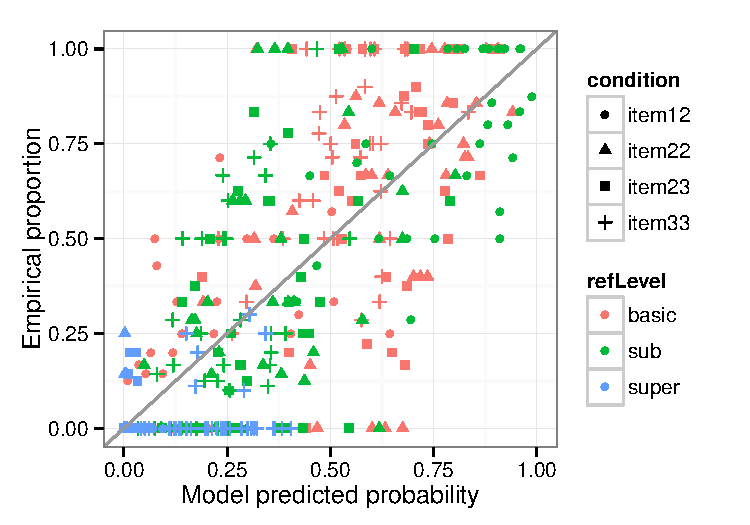
\includegraphics[width=.5\textwidth]{graphs/scatterplot}
%\caption{Mean empirical production data for each level of reference against the MAP of the model posterior predictive at the by-target level.}
% \label{fig:scatterplot}
%\end{figure}

%Point-wise maximum a posteriori (MAP) estimates of the model's posterior predictives at the target level (collapsing across distractors for each target, within each condition) are compared to empirical data in Fig.~\ref{fig:scatterplot}. On the by-target level the model achieves a correlation of $r = .79$. Looking at results on the by-domain level (collapsing across targets) and on the by-condition level (further collapsing across domains, as in \figref{fig:qualitativemodel}) yields correlations of .88 and .96, respectively. 
%The model does a good job of capturing the quantitative patterns in the data, especially considering the sparsity of our data at the by-target level.
%One clear flaw is that the model predicts greater use of the super level label than people exhibit.
%Further systematic deviation appears likely for specific items. 
%On examination, candy items like ``gummy bears'' or ``jelly beans'' were particularly problematic, being referred to primarily by their sub level term in all contexts.

%\begin{figure}
%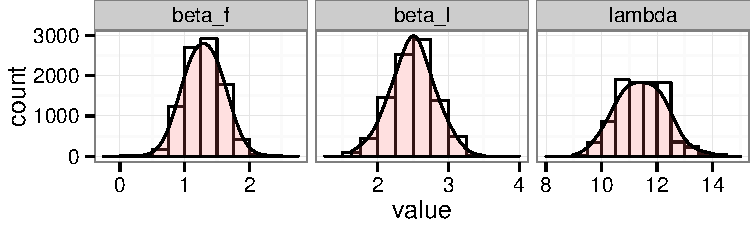
\includegraphics[width=.49\textwidth]{graphs/parameterposteriors.pdf}
%\caption{Posterior distribution over model parameters. Maximum a posteriori (MAP) $\lambda = 10.8$, 95\% highest density interval (HDI) $= [9.7, 12.8]$; MAP $\beta_l = 2.5$, HDI $= [1.9, 3.1]$; MAP $\beta_f = 1.3$, HDI $= [0.8, 1.8]$.}
%\label{fig:paramposteriors}
%\end{figure}

%Parameter posteriors are presented in Fig.~\ref{fig:paramposteriors}. 
%Informativeness is weighted relatively strongly, while length is weighted somewhat more strongly than frequency.
%Note that the 95\% highest density intervals (HDIs) for all three weight parameters exclude zero, indicating that some contribution of each is useful in explaining the data.
%In order to ascertain whether typicality was indeed contributing to the explanatory power of the model, we ran an additional Bayesian data analysis with an added typicality weight parameter $\beta_t \in [0,1]$. This parameter interpolated between empirical typicality values (when $\beta_t {=} 1$) and deterministic (i.e. $0$ or $1$) \emph{a priori} values based on the true taxonomy (when $\beta_t {=} 0$).
%We found a MAP estimate for $\beta_t$ of $.94$, HDI $= [0.88,1]$, strongly indicating that it is useful to incorporate empirical typicality values.
%Finally, we ran a model including a parameter weighting the \emph{product} of frequency and cost, corresponding to the interaction term in our regression analysis. Its posterior distribution was strongly peaked at 0, indicating that any contribution of the interaction is already captured by other aspects of the model. 



\section{\bf Discussion and conclusion}

%The choice speakers make of how to refer to an object is influenced by a rich variety of factors.
%In this paper, we specifically investigated the choice of level of reference in nominal referring expressions. In an interactive reference game task in which speakers freely produced referring expressions, utterance choice was affected by utterance cost (in terms of length and frequency), contextual informativeness (as manipulated via distractor objects), and object typicality.
%The interplay of these factors is naturally modeled within the RSA framework, where speakers are treated as choosing utterances by soft-maximizing utterance utility, which includes terms for informativeness and cost. In previous formulations of RSA models, informativeness was determined by a deterministic semantics; here we ``softened'' the semantics by allowing nouns to apply to objects to the extent that those objects were rated as typical for the nouns.
%The resulting model provided a good fit to speakers' empirical utterance choices, both qualitatively and quantitatively. 
%The model predicts a well-documented preference for speakers  to refer to objects at the basic level when not constrained by contextual considerations  \cite{RoschEtAl76_BasicLevel}. In our model, this preference emerges naturally from cost considerations: basic-level labels tend to be shorter and more frequent than sub and super level terms. However, speakers did not always use the basic level term, even when unconstrained by context. In certain cases where object typicality was relatively high for the sub level term compared to the basic level term, that term was preferred (as was the case for ``panda bear''), suggesting an interesting interplay between typicality and level of description. 
%While our results show that a model can capture several basic-level phenomena through frequency, length, and typicality features, it leaves open the origin and causal role of these linguistic regularities.
%Future research will be needed to determine how linguistic regularities are related to conceptual regularities and why.
%An interesting analogy can be drawn from choosing a noun to choosing a set of adjectives; that is, between selection of a level of reference in simple nominal referring expressions and selection of a set of features to include in modified referring expressions. 
%For the latter, a much discussed phenomenon is that of \emph{overinformative} modifier use \cite{Gatt2014}---for example, saying ``big blue'' when all objects in the context are blue. 
%The preference for the basic level in the \emph{super sufficient} condition and the still substantial use of sub level terms in the \emph{basic sufficient} condition can also be considered overinformative. However, we showed that a Rational Speech-Acts model using non-deterministic semantics, derived from typicality estimates, predicts that speakers \emph{should} use these more specific descriptions. 
%The extent to which similar considerations may apply to modified referring expressions should be explored.
%Future research should also examine the interaction of these choices: circumstances under which speakers choose a modifier and how nominal and modifier choice interact.

\section{\bf Acknowledgments}
\small
This work was supported by ONR grant N00014-13-1-0788 and a James S. McDonnell Foundation Scholar Award to NDG and an SNF Early Postdoc.~Mobility Award to JD. RXDH was supported by the Stanford Graduate Fellowship and the National Science Foundation Graduate Research Fellowship under Grant No. DGE-114747.



\bibliographystyle{apacite}

\setlength{\bibleftmargin}{.125in}
\setlength{\bibindent}{-\bibleftmargin}

\bibliography{bibs}


\end{document}